\documentclass{beamer}

\usetheme{Madrid}

\usepackage{graphicx}
\usepackage{amsmath,amssymb}
\usepackage{caption}

\DeclareMathOperator{\E}{\mathbb{E}}
\captionsetup[figure]{labelformat=empty}

\title[]{The Impact of Imputation Quality on Family-Based Analysis}
\author[]{Mahdi Mir (UCLA \& SSGAC) \\ Alexander S. Young (UCLA \& SSGAC)}
\date[]{Oct 2024}

\begin{document}

\maketitle


\begin{frame}{Imputation from a Reference Panel}
      % First, I give a brief introduction to imputation.

      % Imputation in general is a process in which we predict the genotypes that are not directly observed.

      % also we use a reference panel to predict the genotypes that are not directly observed.

      % this figure is from Zheng et al. (2011) is a good visual representation of the imputation process.
      % suppose we a have reference panel and we have some genotypes that are directly observed and also we have some genotypes that are not directly observed.
      % in the imputation process we are going to use the information from the reference panel and the observed genotypes to predict the unobserved genotypes.
      % the predicted genotypes are called imputed genotypes.
      % for the genotyps that we don't know we can have best guess for them or we can have a range of possible genotypes.
      % we can have a probability distribution for the genotypes that we don't know.
      \begin{figure}
            \centering
            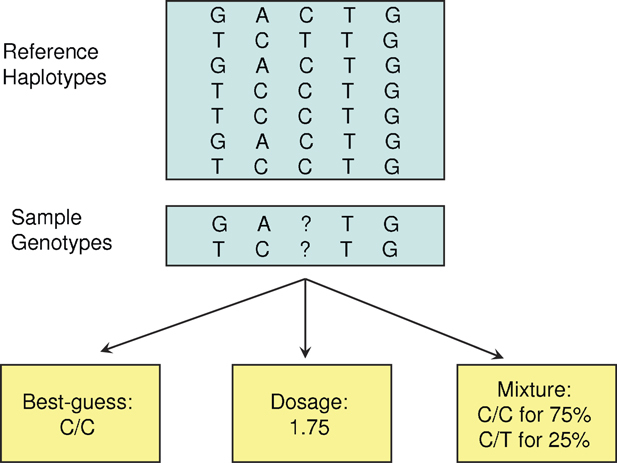
\includegraphics[width= .63\textwidth]{fig/mfig001-2.jpg}
      \end{figure}
      \begin{center}
            \(\text{Hard Call}=\text{Best Guess}\) \hspace{25pt}  \(\text{Dosages}=\E[\hat{G}]\)
            \\
            \vspace{5pt}
            \(0 \leq \text{Info Score} \leq 1\) \(\quad\) \(\uparrow\) Imputation Quality \(\Longleftrightarrow\) \(\uparrow\) Info Score
      \end{center}
      \rule{0.3\linewidth}{0.4pt}
      \\
      \tiny{Source: Zheng et al. (2011)}

      % the takeaway from this slide is that what is imputation: we just fill in the gaps in the data using a reference panel.
      % and what is the info score: it is the quliay of the imputation. that is a number between 0 and 1. the higher the the more qulity the imputation is.

\end{frame}

\begin{frame}{Reference Based Imputation VS Mandelian Imputation}
      \begin{itemize}
            % oversell the paper of Alex and talk about the package.
            \item Mandellian imputation as done in SNIPAR (Young et.al, Nature Genetics 2022) is very different from reference based imputation.
            % Imputation from a reference panel is filling variants according to a reference panel for a single individual.
            % Mandellian imputation is used in family based analysis to fill in the genotypes of the parents based on the genotypes of the offspring.
            % in fact these are different methods that are used for different purposes and applications and are very different.
            \vspace{15pt}
            \item Reference based imputation is not taking into account the relationships between the individuals.
            % This allows us to have more data points for our studies, leading to potentially stronger conclusions.
            % \item Imputation is used in GWAS to increase the power of the study and to increase the number of SNPs that are available for analysis.
            % % Highlight how this contributes to the overall strength of genetic studies.
      \end{itemize}
\end{frame}

\begin{frame}{Motivation}
      \begin{itemize}
            \item Family-based research designs rely on special properties of the data.
            % that might not be preserved in low-quality imputed genotypes.
            \vspace{15 pt}
            % We are concerned that
            \item Low-quality imputed genotypes may not work for family-based analysis. % and maybe for other types of analysis
            \vspace{15 pt}
            % We are interesed in understanding the impact of imputation quality on downstream analysis by comparing to the WGS data.
            \item Understanding the impact of imputation quality on downstream analysis by comparing to the WGS data
            % item E.g.: In theory by the Mendelian laws we expect the correlation between sibling pairs and parent-offspring pairs genotypes to be 0.5.
            % Reinforce the idea that expectations are based on genetic principles.
            % \item Current imputation methods do not take into account the relationships between the individuals.
      \end{itemize}
\end{frame}

% In this part, we have some figures that effectively convey our point.
% Each step of the analysis has its own challenges, but we won't go into too much technical detail here.

\begin{frame}{Correlation Analysis in UK Biobank}
      \begin{itemize}
            \item UK Biobank Imputed Data
            \vspace{10pt}
            \begin{itemize}
                  % our sample is restricted to white British subsample.
                  \item White British subsample
                  \vspace{10pt}
                  \item \(19K\) sibling pairs
                  \vspace{10pt}
                  \item \(4K\) parent-offspring pairs
                  \vspace{10pt}
                  \item SNPs with \(MAF>1\%\) and  % so we don't have rare variants in our analysis.
            \end{itemize}
      \vspace{15pt}
      % our sample selection corresponds to the sample used in Howe et.al (2022) Sib-GWAS paper.
      \item Howe et.al (2022) Sib-GWAS used Hard-Calls low-quality (Info Score \(> 0.3\)) imputed SNPs. % in their analysis and that can be an issue.
      \end{itemize}
\end{frame}

\begin{frame}{Correlations Distribution - Full Siblings}
      % first explain the figures then intrepret them. 
      % interpreatation of the figures.
      \begin{columns}
            \begin{column}{0.5\textwidth}
                  \centering
                  \captionof{figure}{Low Quality Imputed}
                  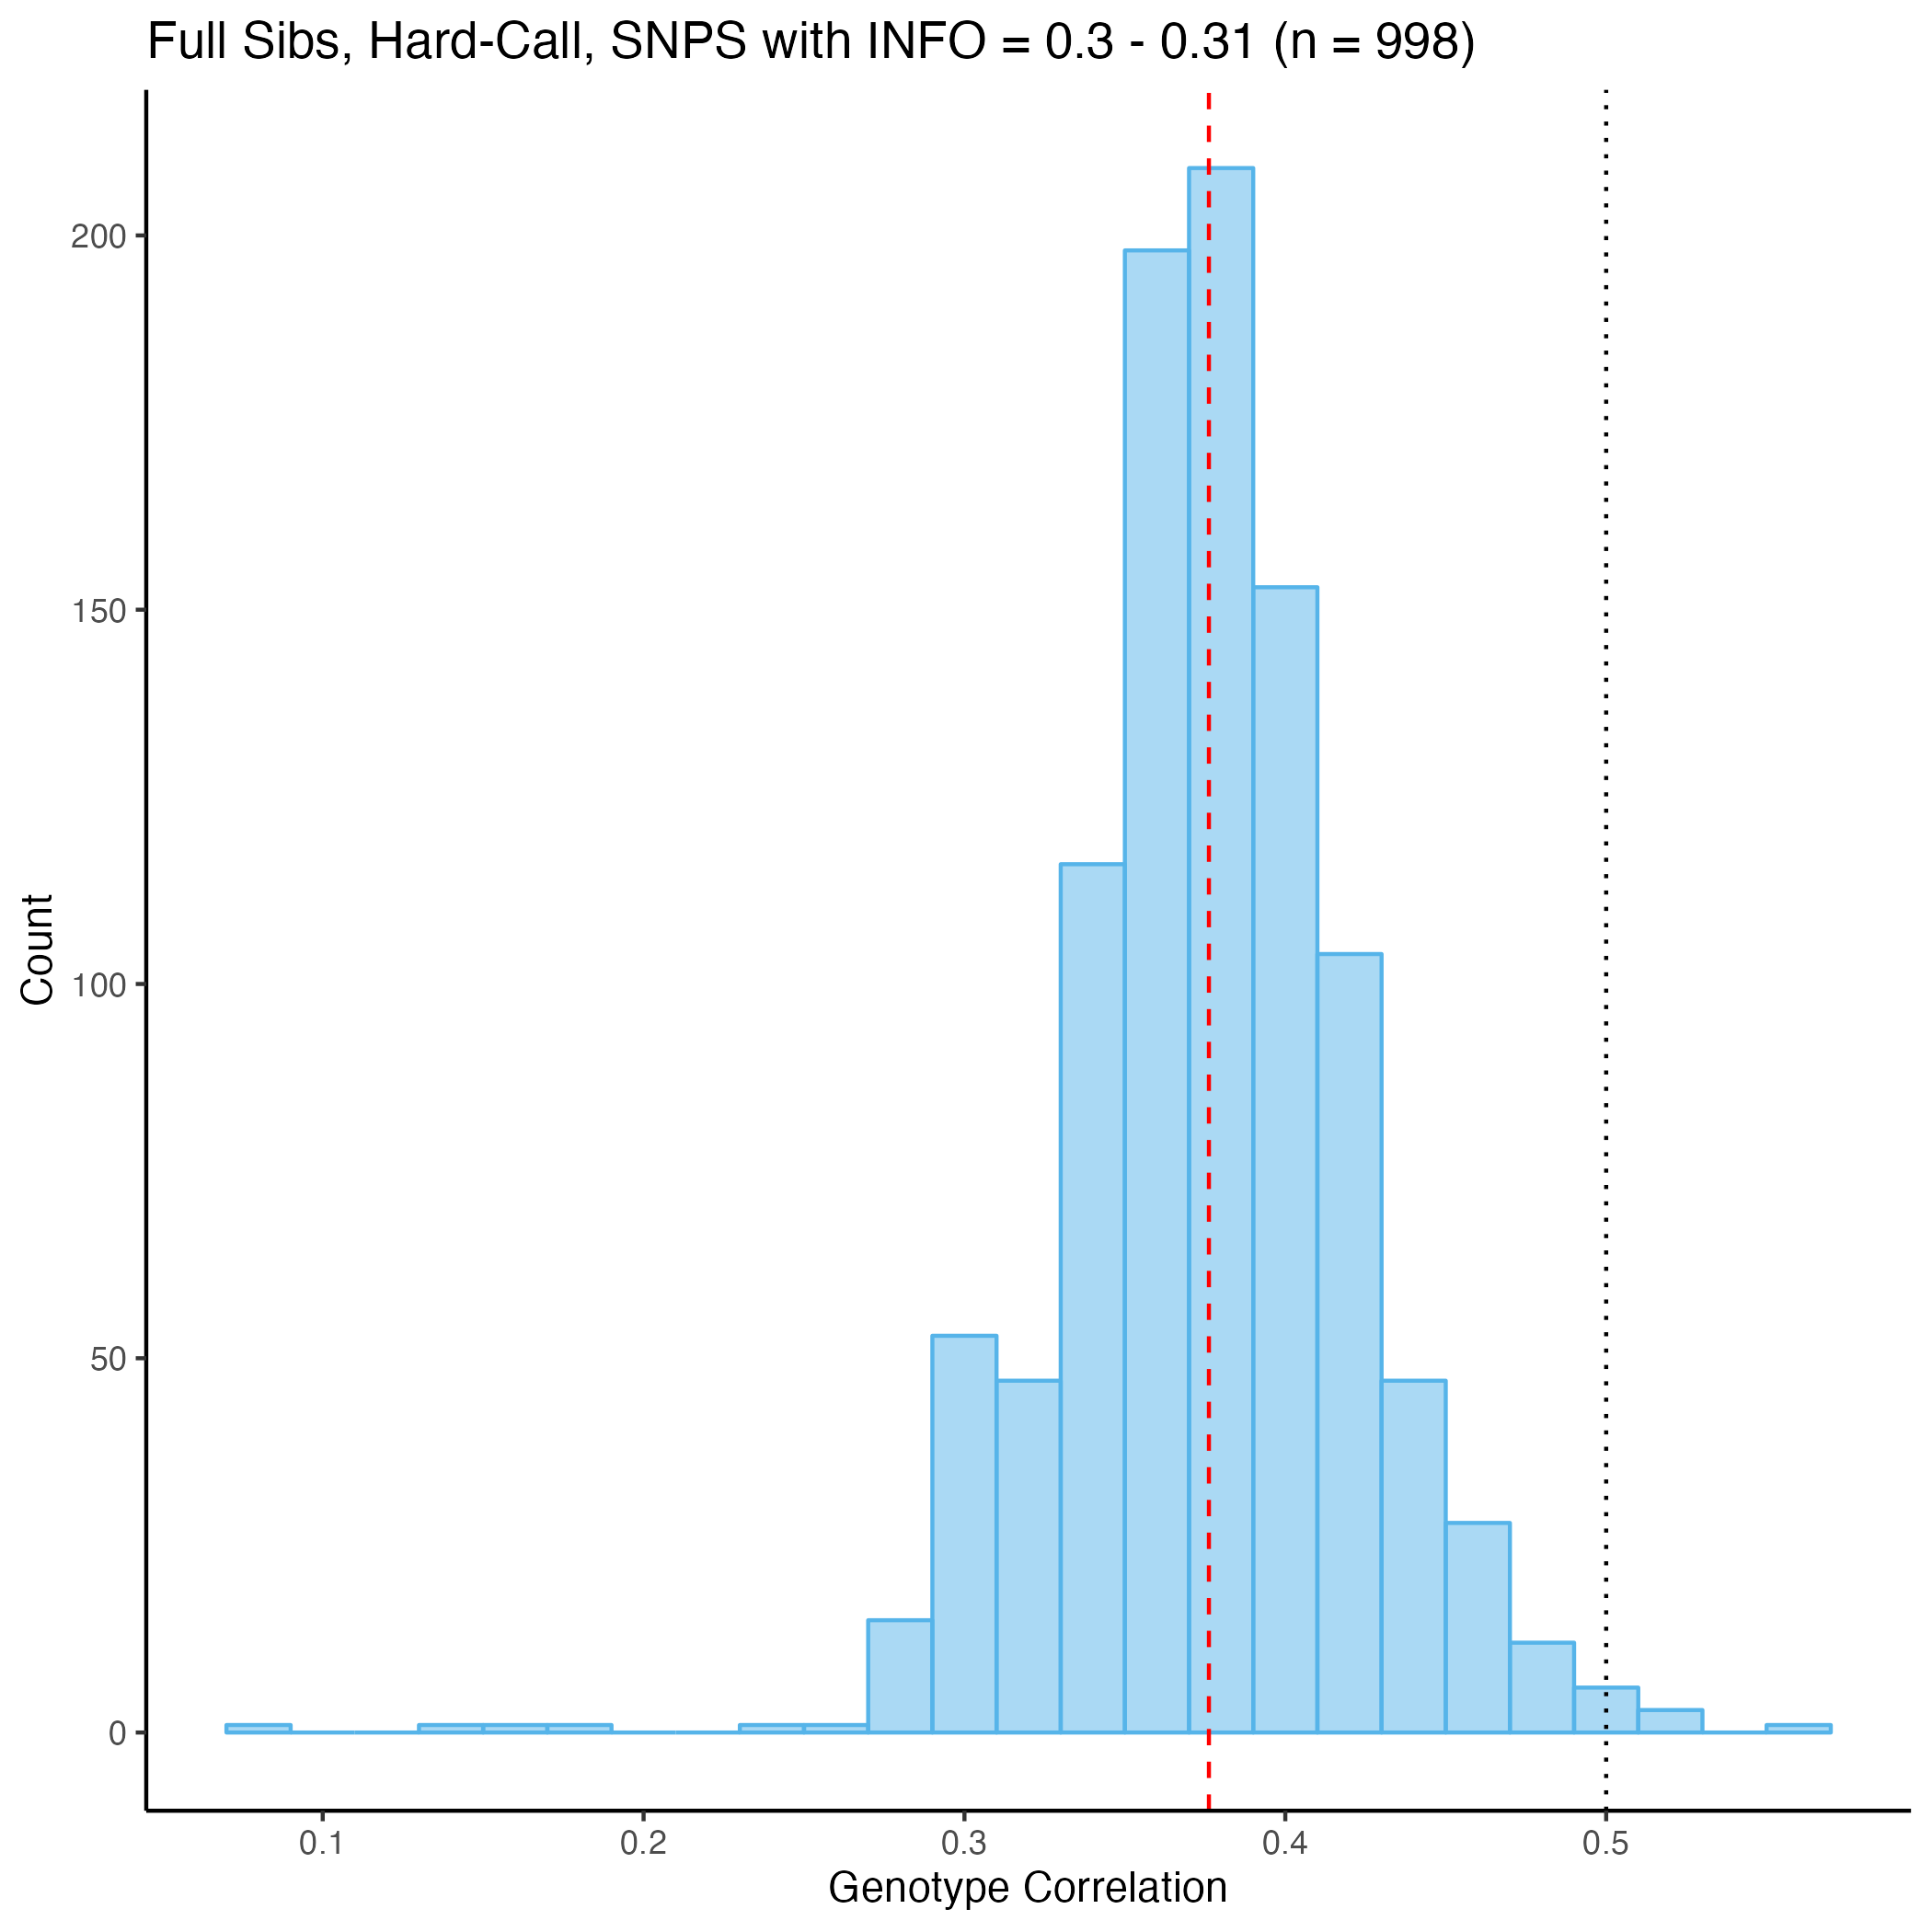
\includegraphics[width= \textwidth]{fig/FS-HC-i30.png}
              \end{column}
            \begin{column}{0.5\textwidth}
                  \centering
                  \captionof{figure}{High Quality Imputed}
                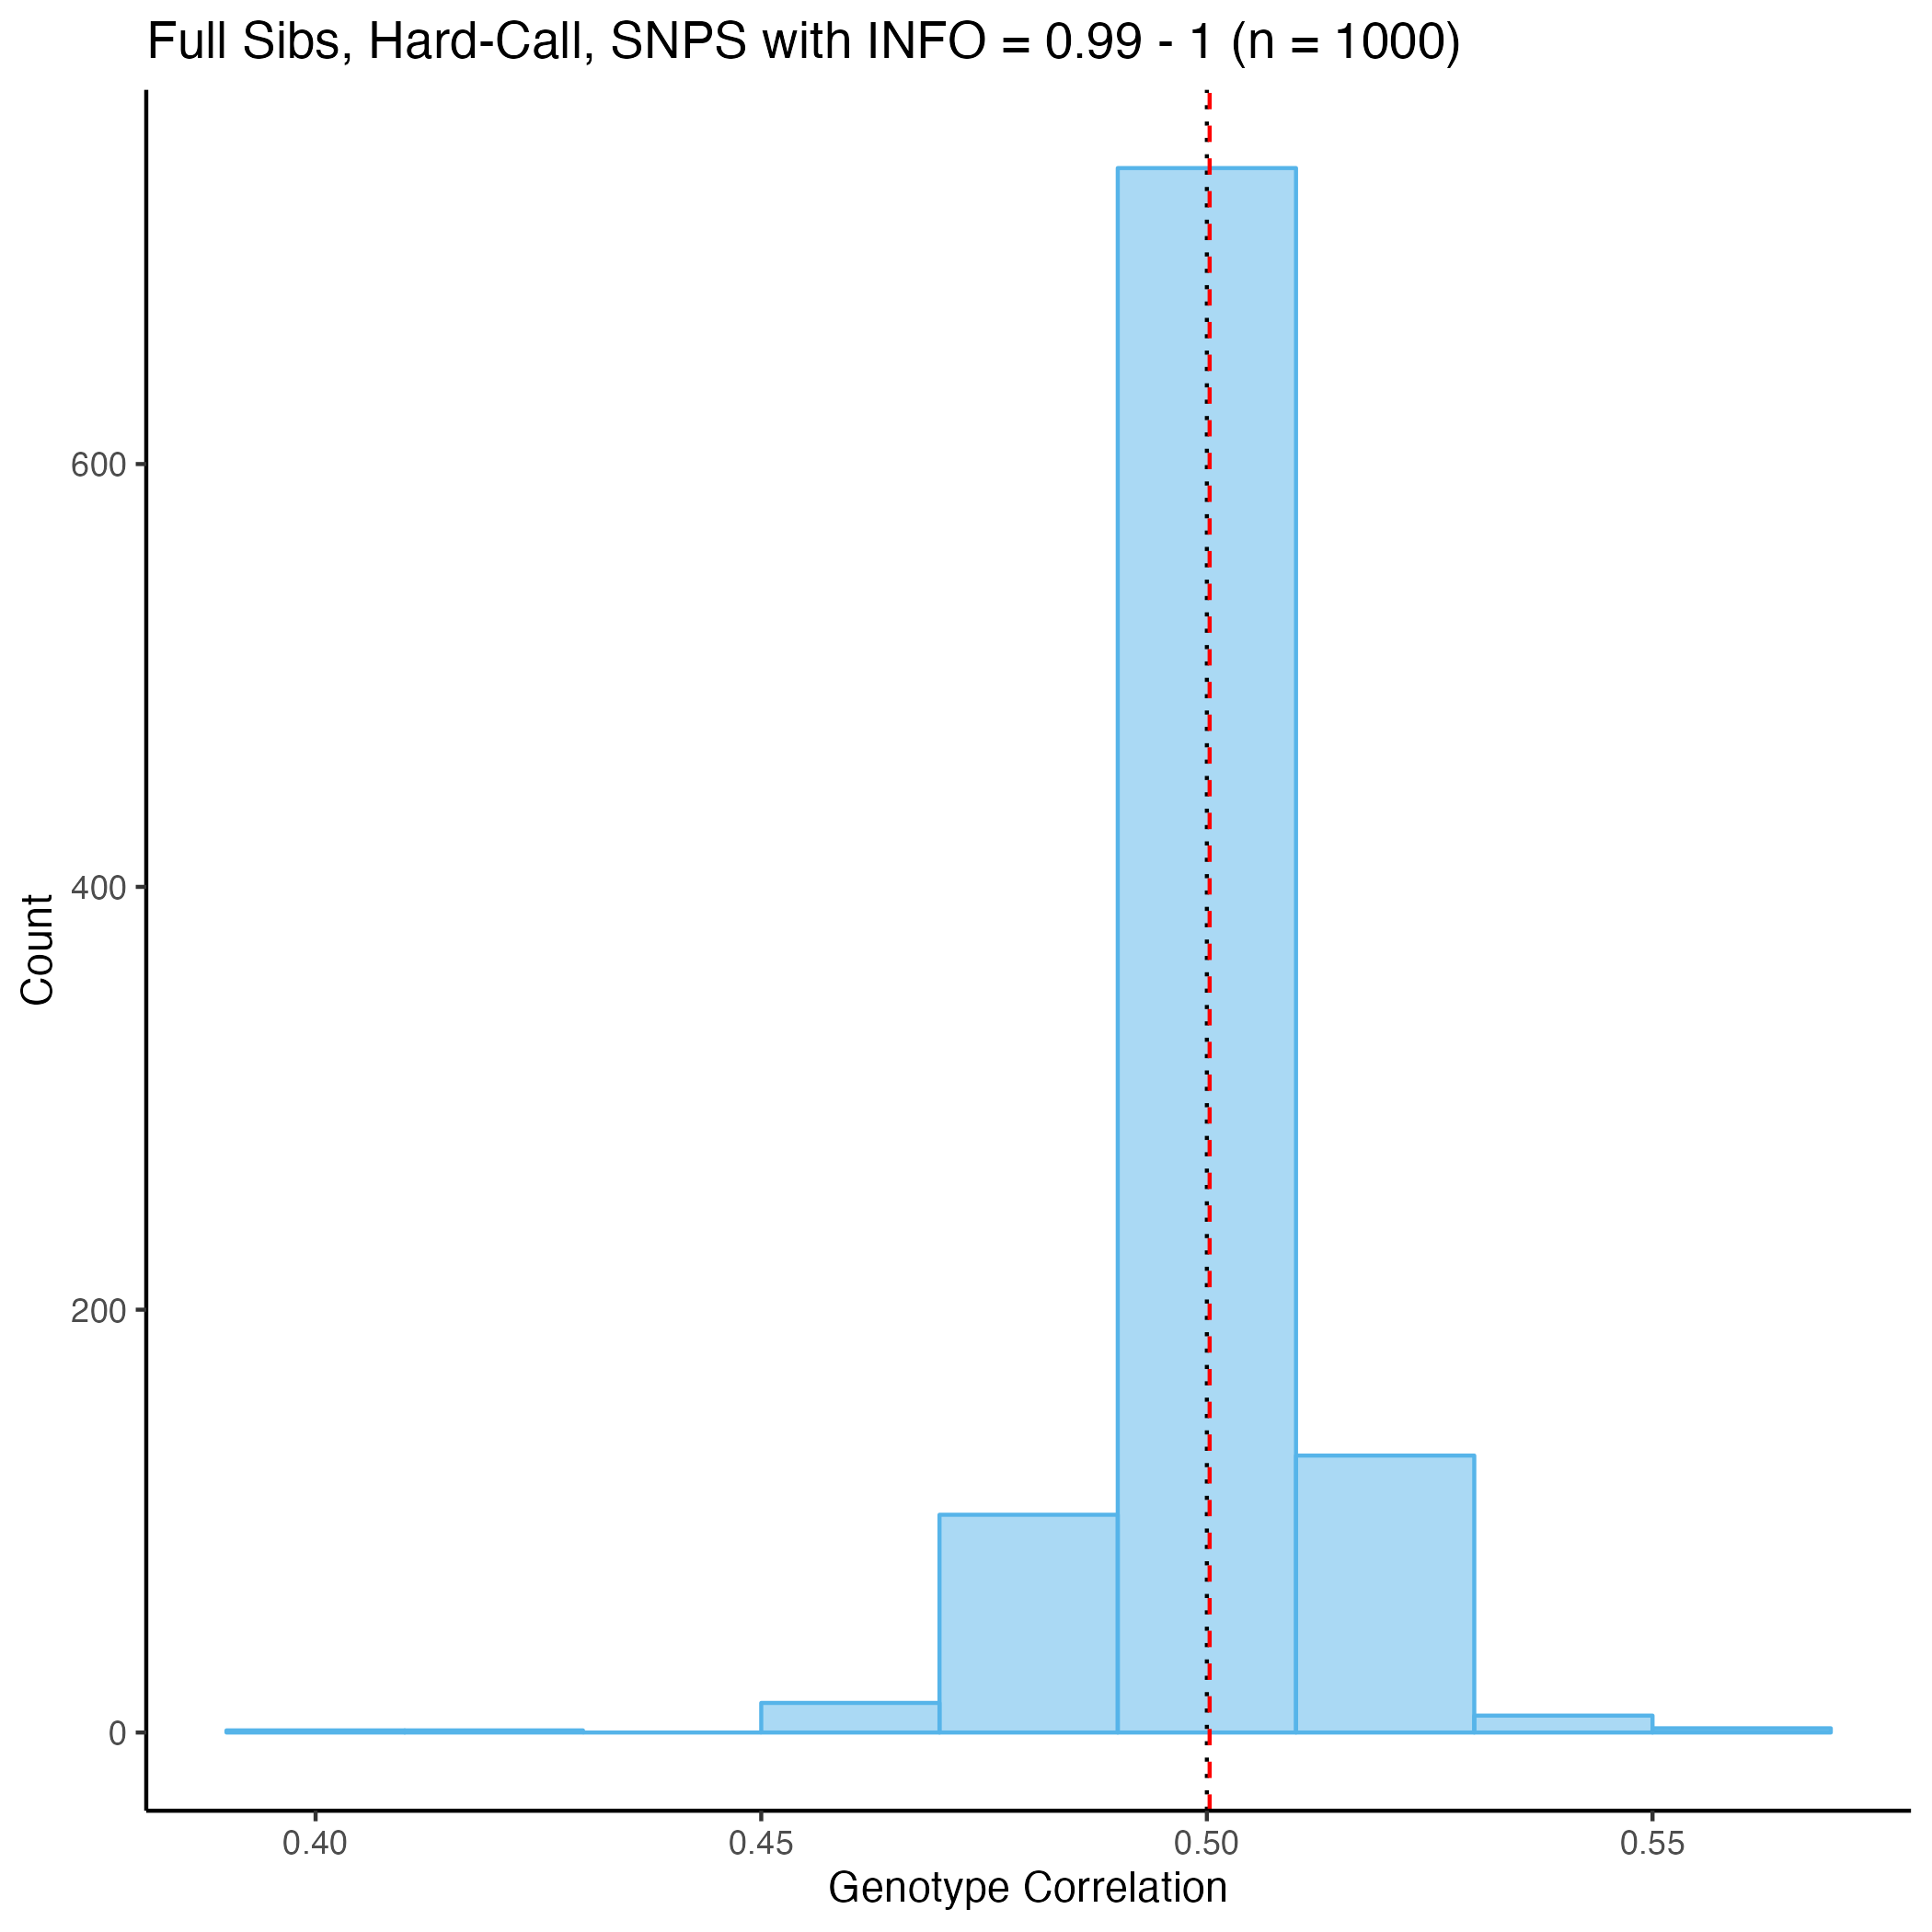
\includegraphics[width= \textwidth]{fig/FS-HC-i99.png}
            \end{column}
        \end{columns}
\end{frame}

\begin{frame}{Correlations Distribution - Parent-Offspring}
      \begin{columns}
            \begin{column}{0.5\textwidth}
                  \centering
                  \captionof{figure}{Low Quality Imputed}
                  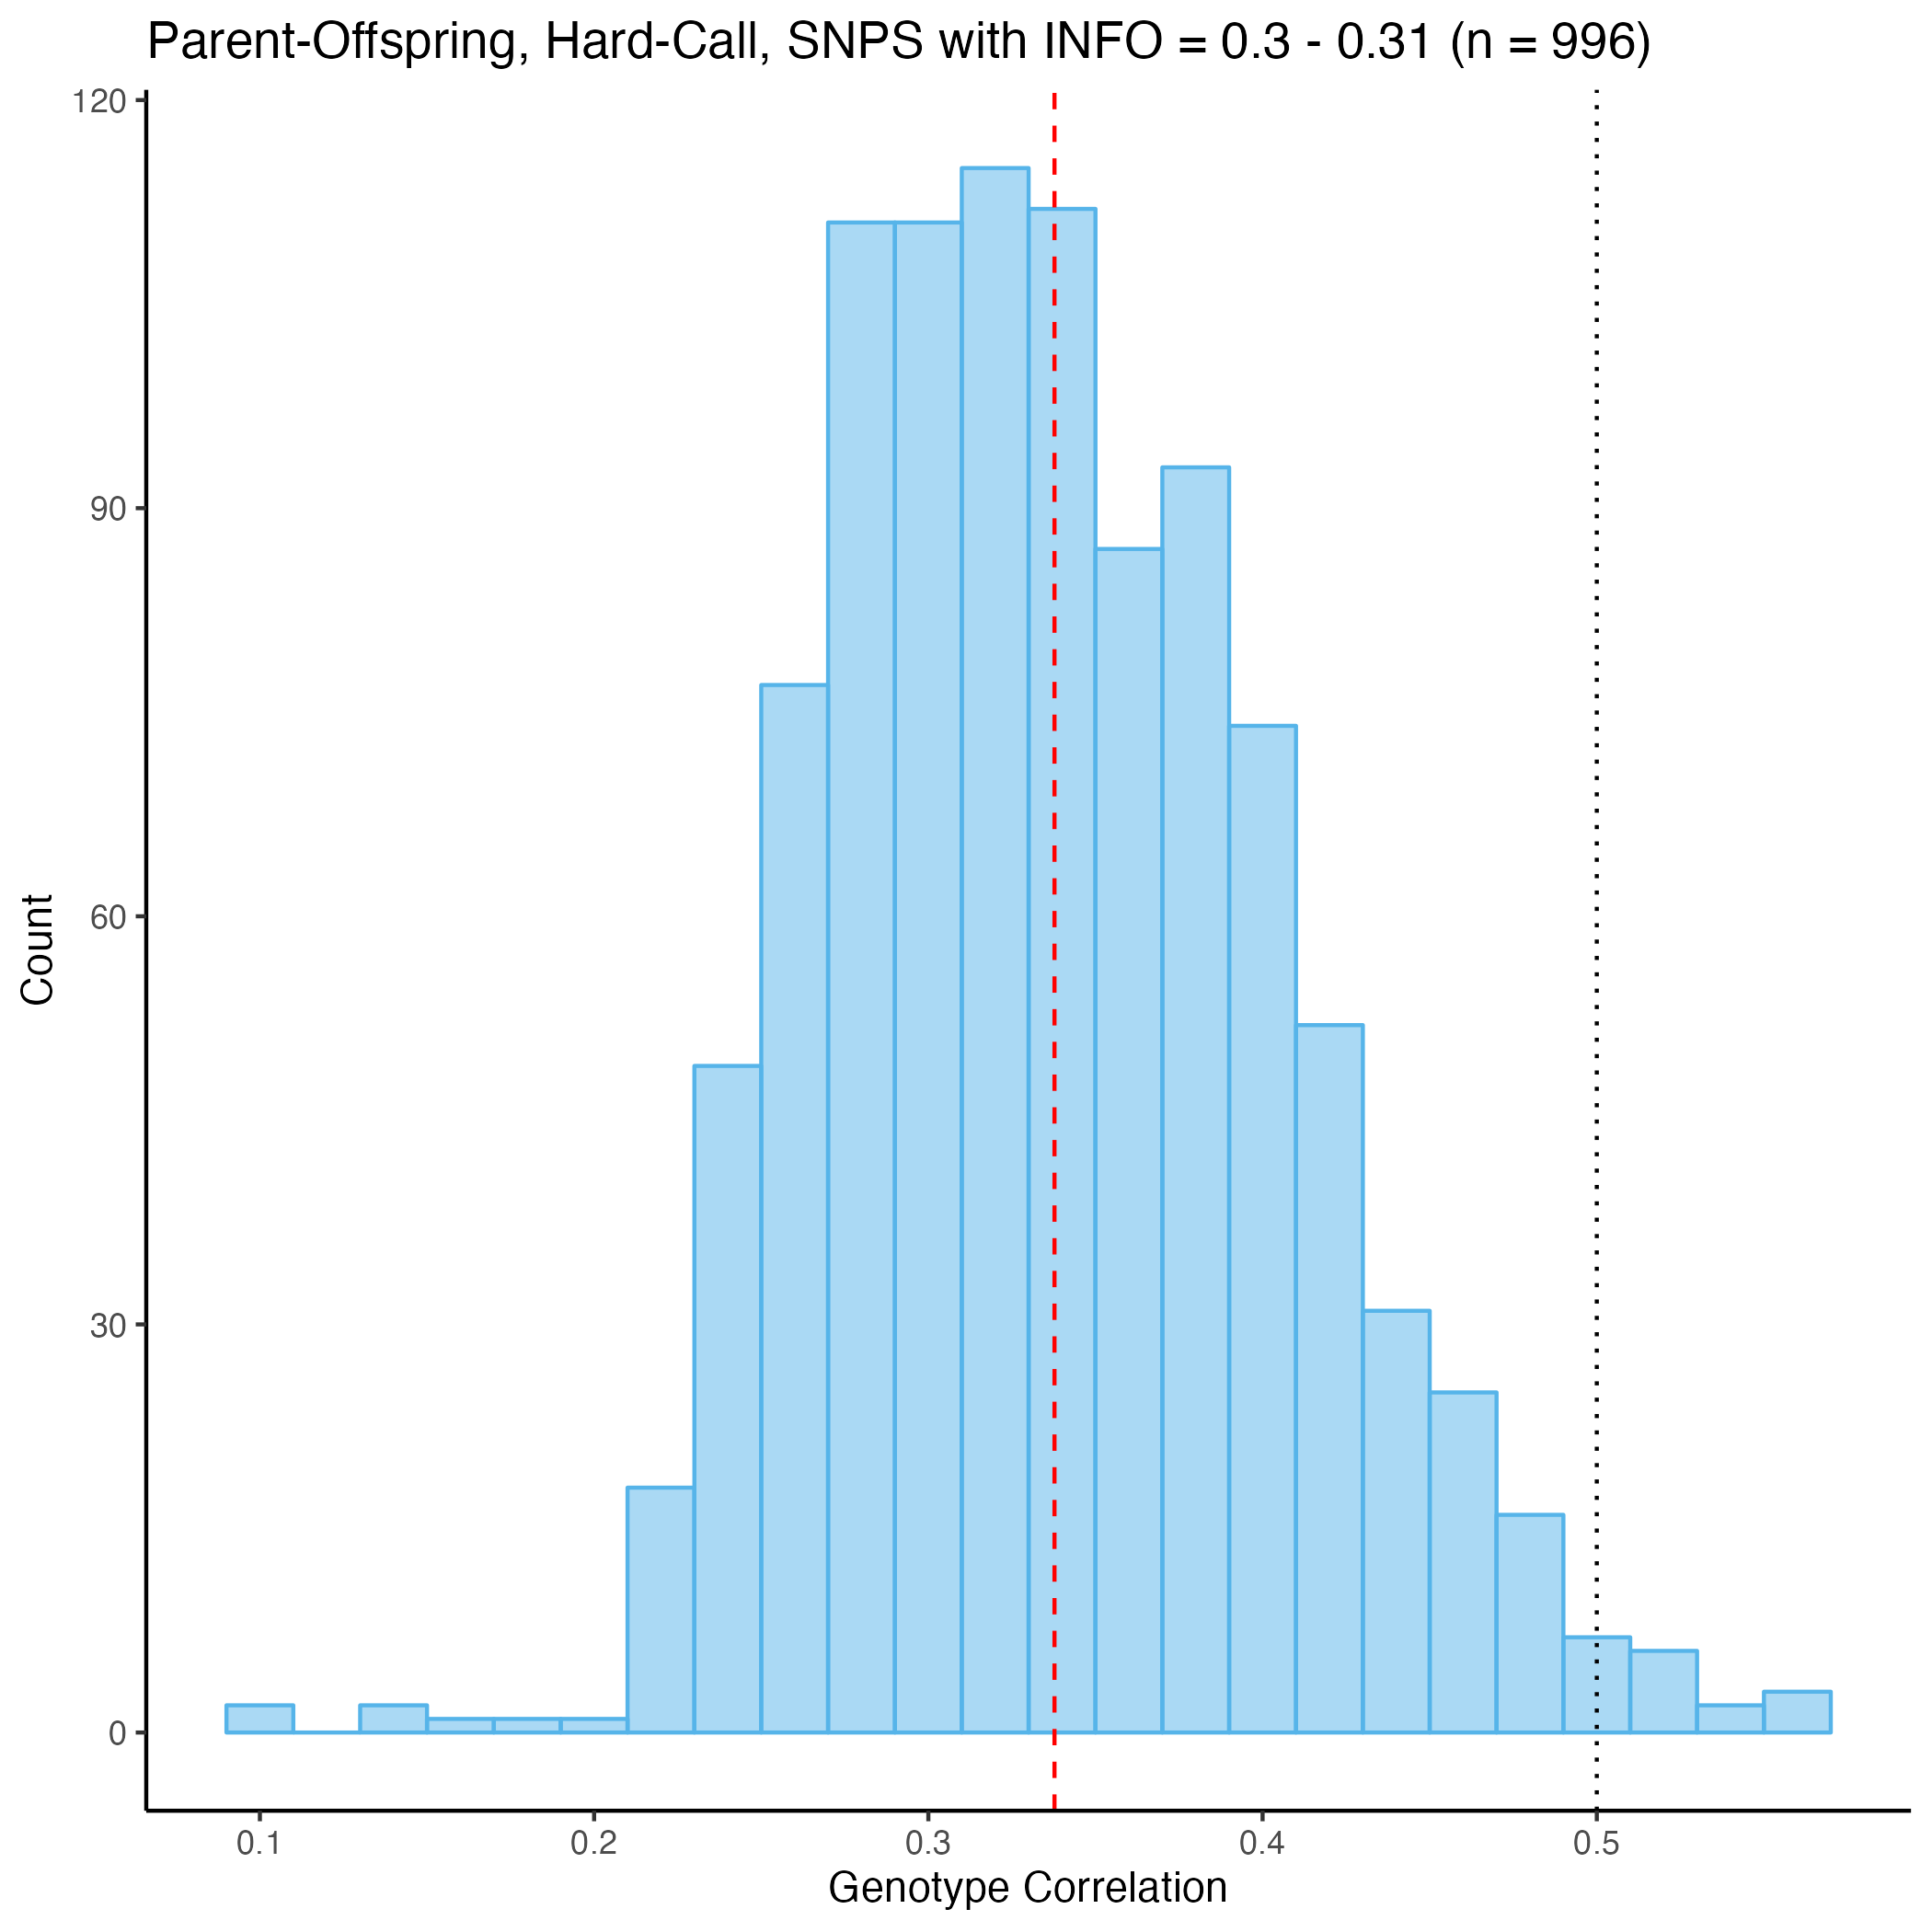
\includegraphics[width= \textwidth]{fig/PO-HC-i30.png}
              \end{column}
            \begin{column}{0.5\textwidth}
                \centering
                \captionof{figure}{High Quality Imputed}
                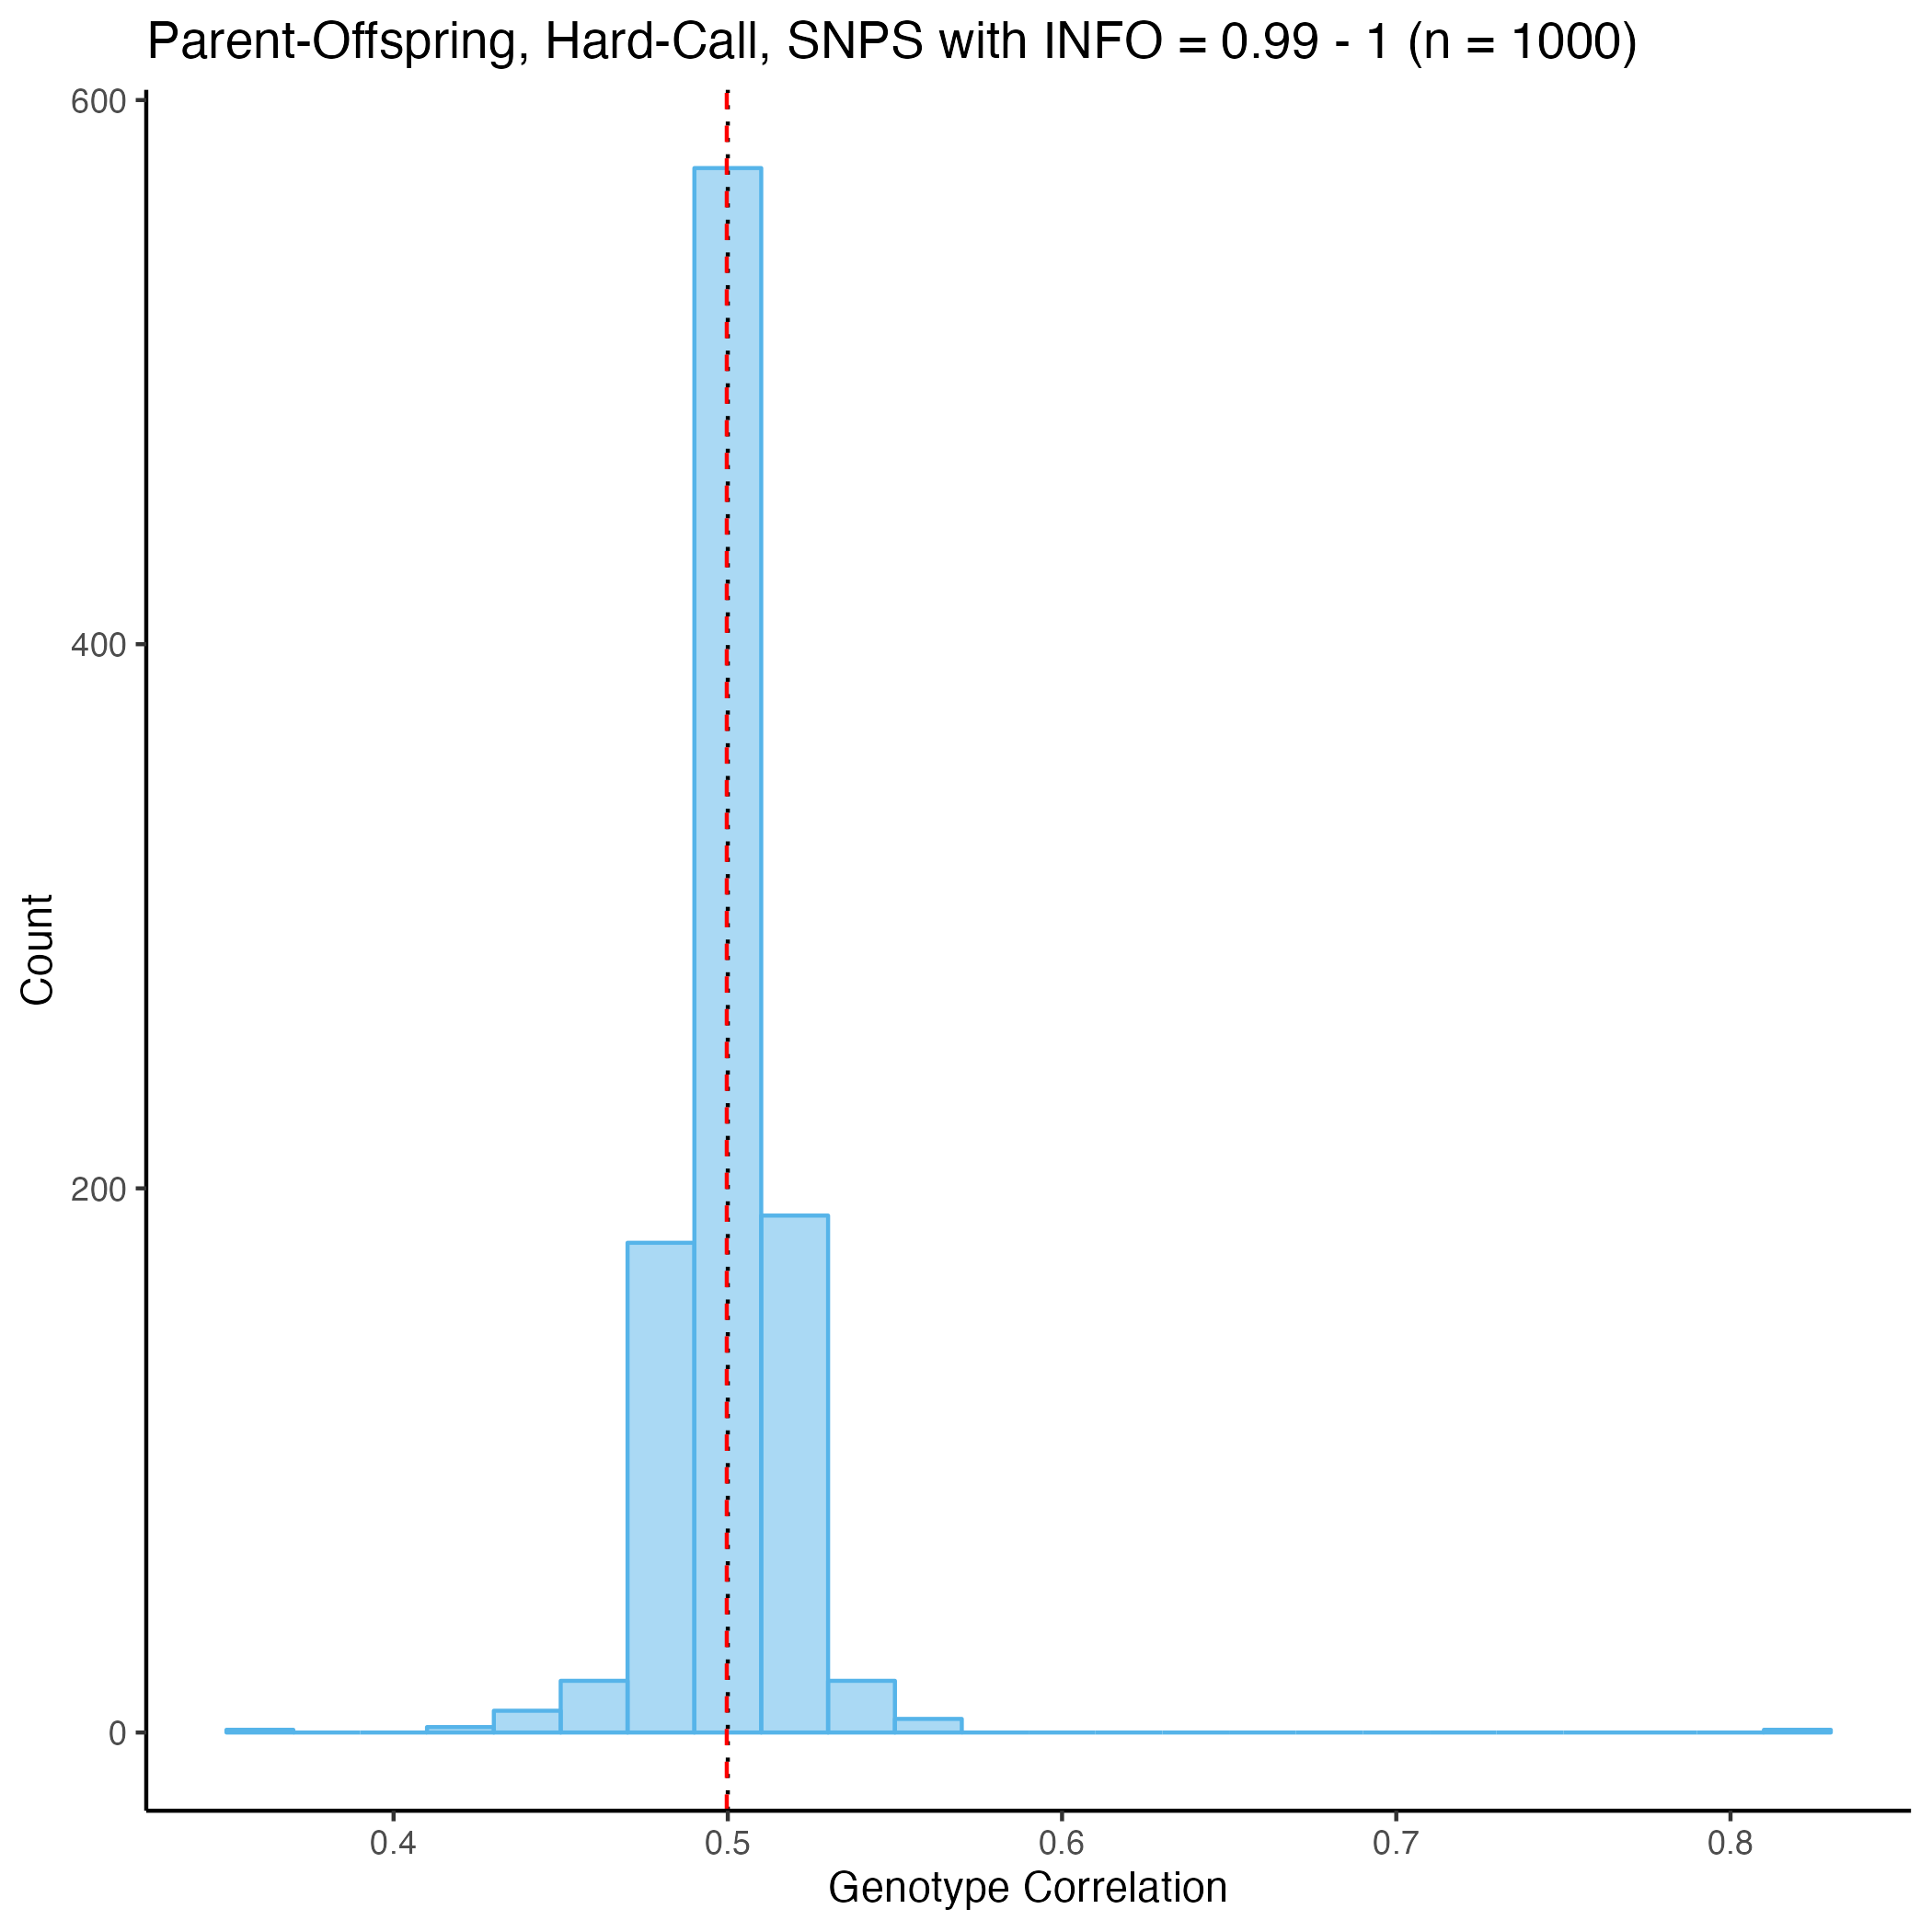
\includegraphics[width= \textwidth]{fig/PO-HC-i99.png}
            \end{column}
        \end{columns}
\end{frame}

\begin{frame}{Mean Genotype Correlation}{As a Function of Info Score}
      \centering
      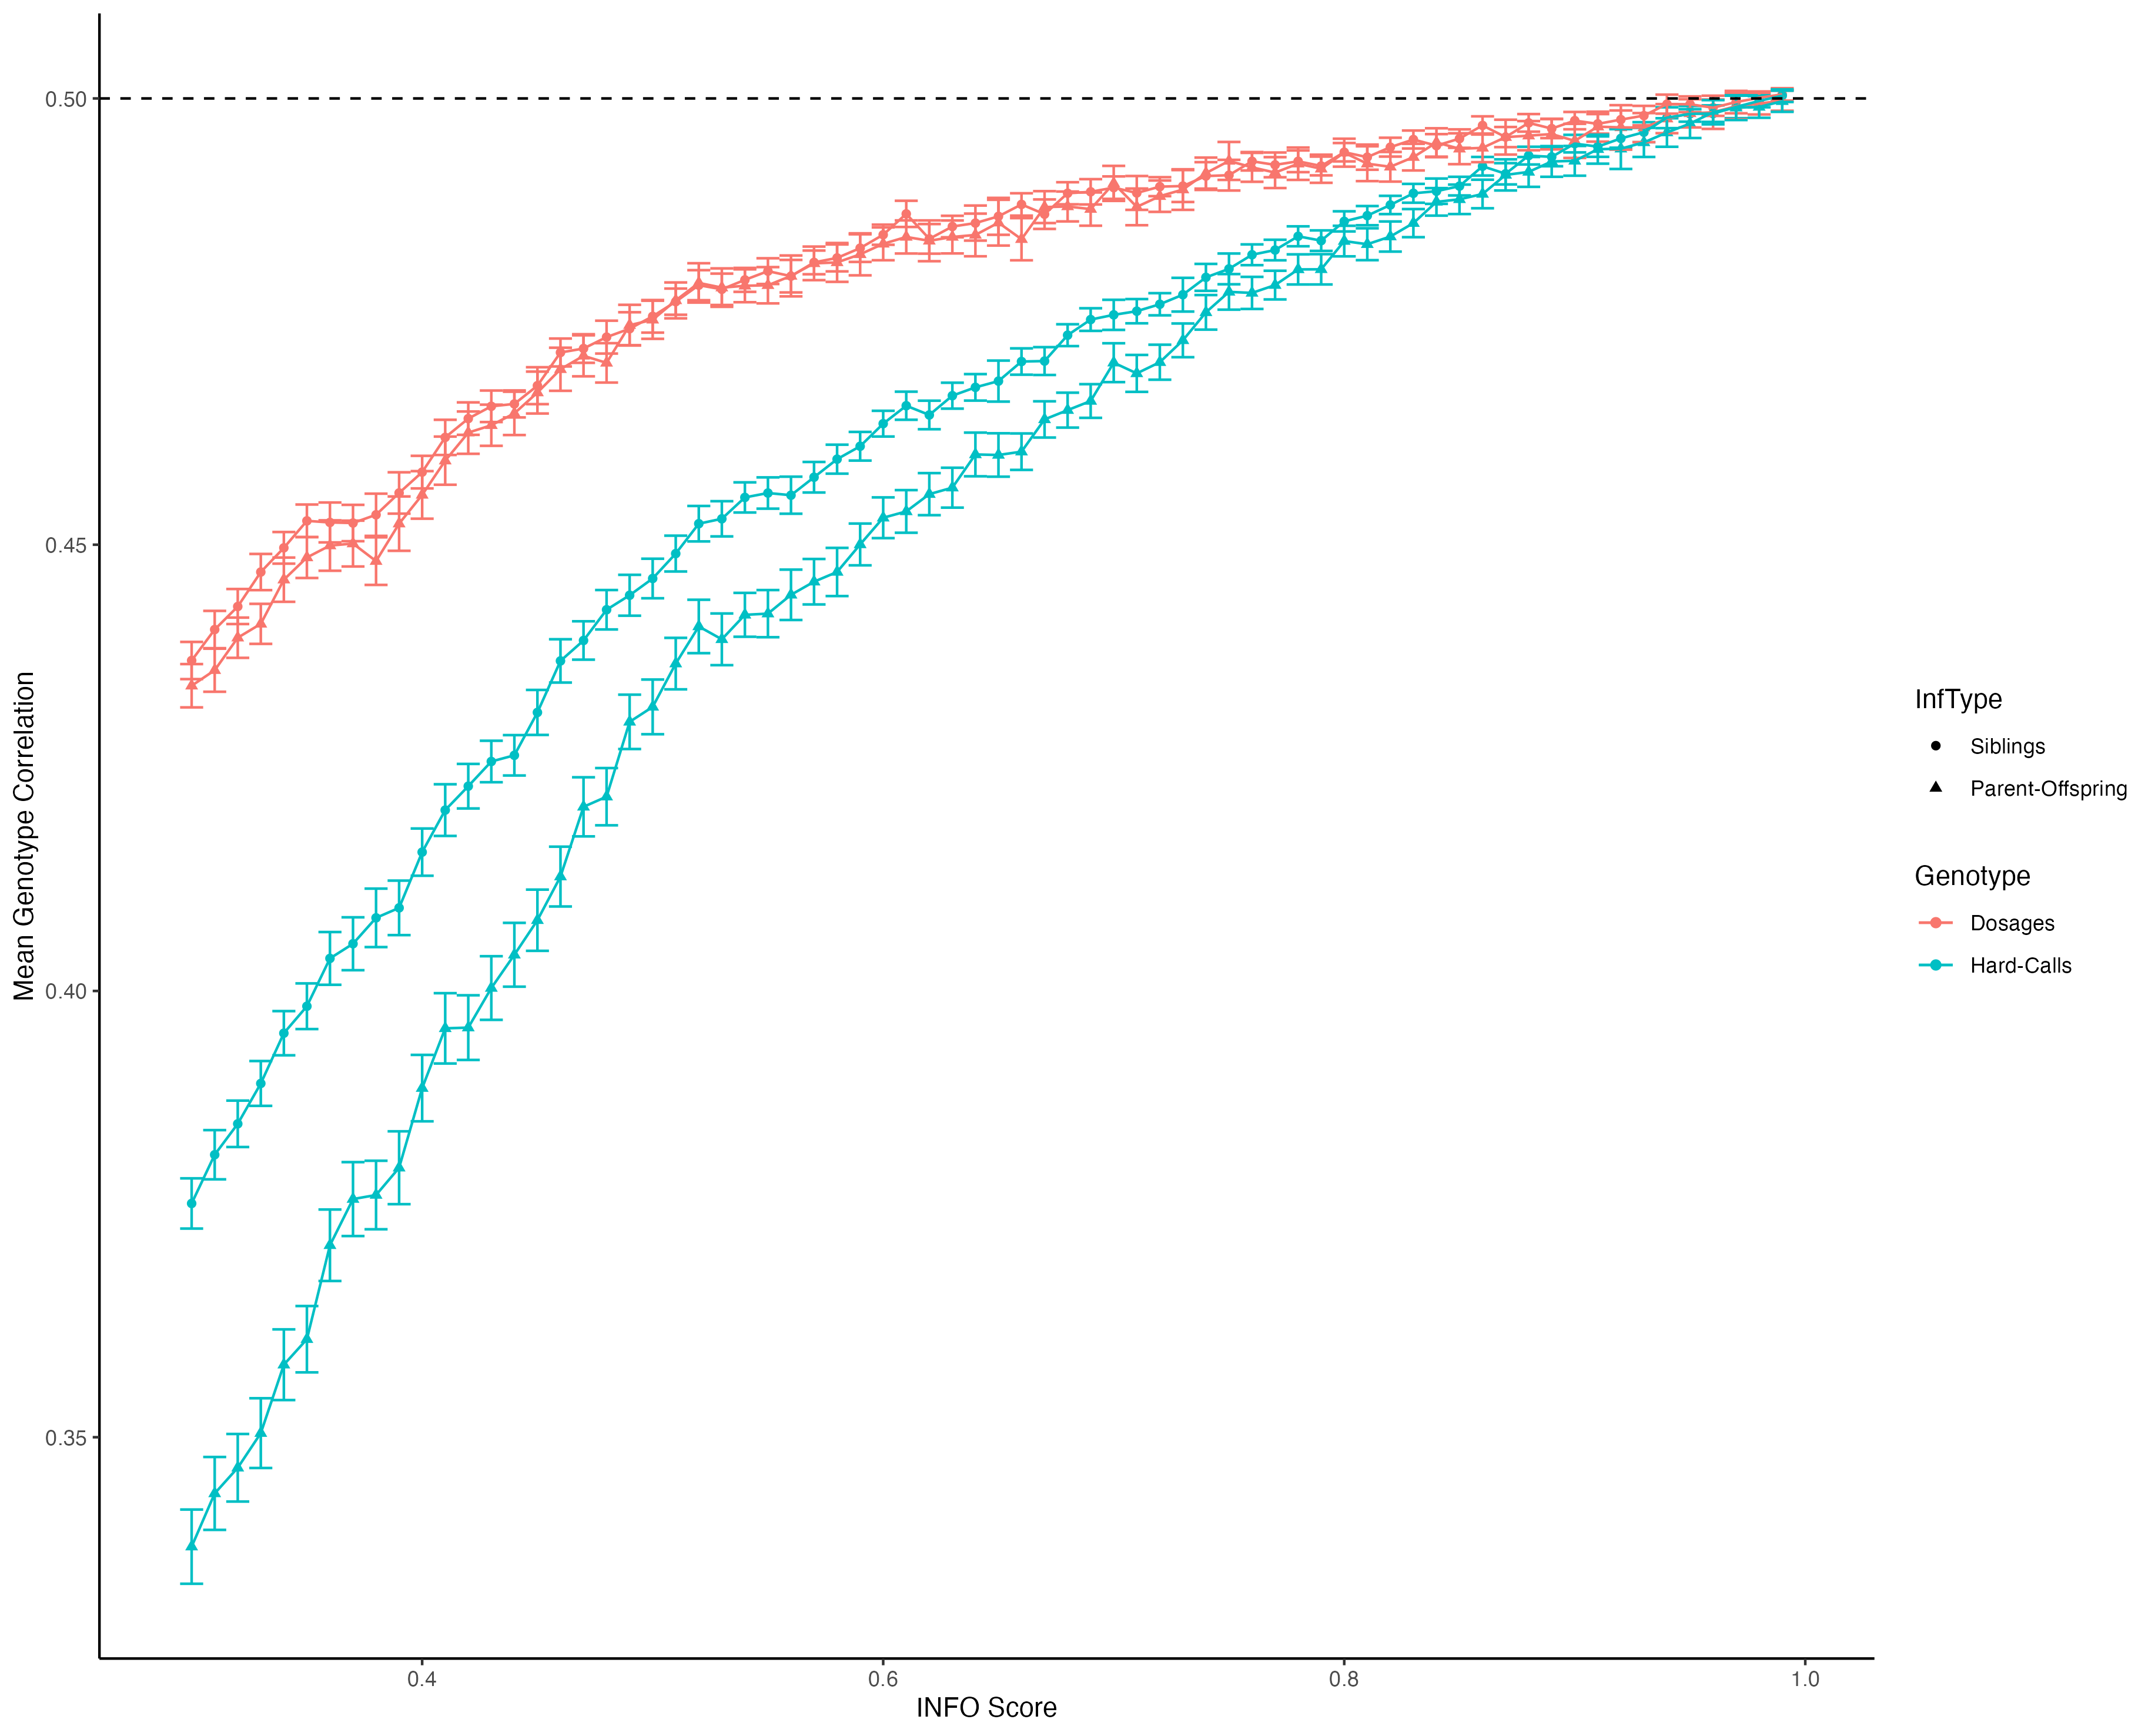
\includegraphics[width=.80\textwidth]{fig/mean_gt_corr_v2.png}
      % Discuss what this graph indicates about the overall quality of imputation.
      % the problem for hard calls is worse than the dosages.
      % the problem for parent-offspring pairs is worse than the sibling pairs.
\end{frame}

\begin{frame}{Correlation Analysis Conditional on IBD states}
      % Explain that the genome is inherited from both parents, affecting sibling correlations.
      \begin{itemize}
            \item Quantitative genetics theory tells us the correlation between siblings' genotypes depends on their IBD state.
            \vspace{15pt}
            \item IBD state records how many allels they share by descent from their parents.
            \vspace{15pt}
            \item Suppose \(i\) and \(j\) are siblings. Then in theory [under random-mating] we have:
      \end{itemize}
      \[
            Corr(G_i, G_j | IBD = 0) = 0
      \]
      \[
            Corr(G_i, G_j | IBD = 1) = 0.5
      \]
      \[
            Corr(G_i, G_j | IBD = 2) = 1
      \]
      % Link these theoretical expectations to your findings and their significance.
\end{frame}

\begin{frame}{Mean Genotypes Correlation Conditional on IBD States}{As a Function of Info Score}
      \begin{figure}
            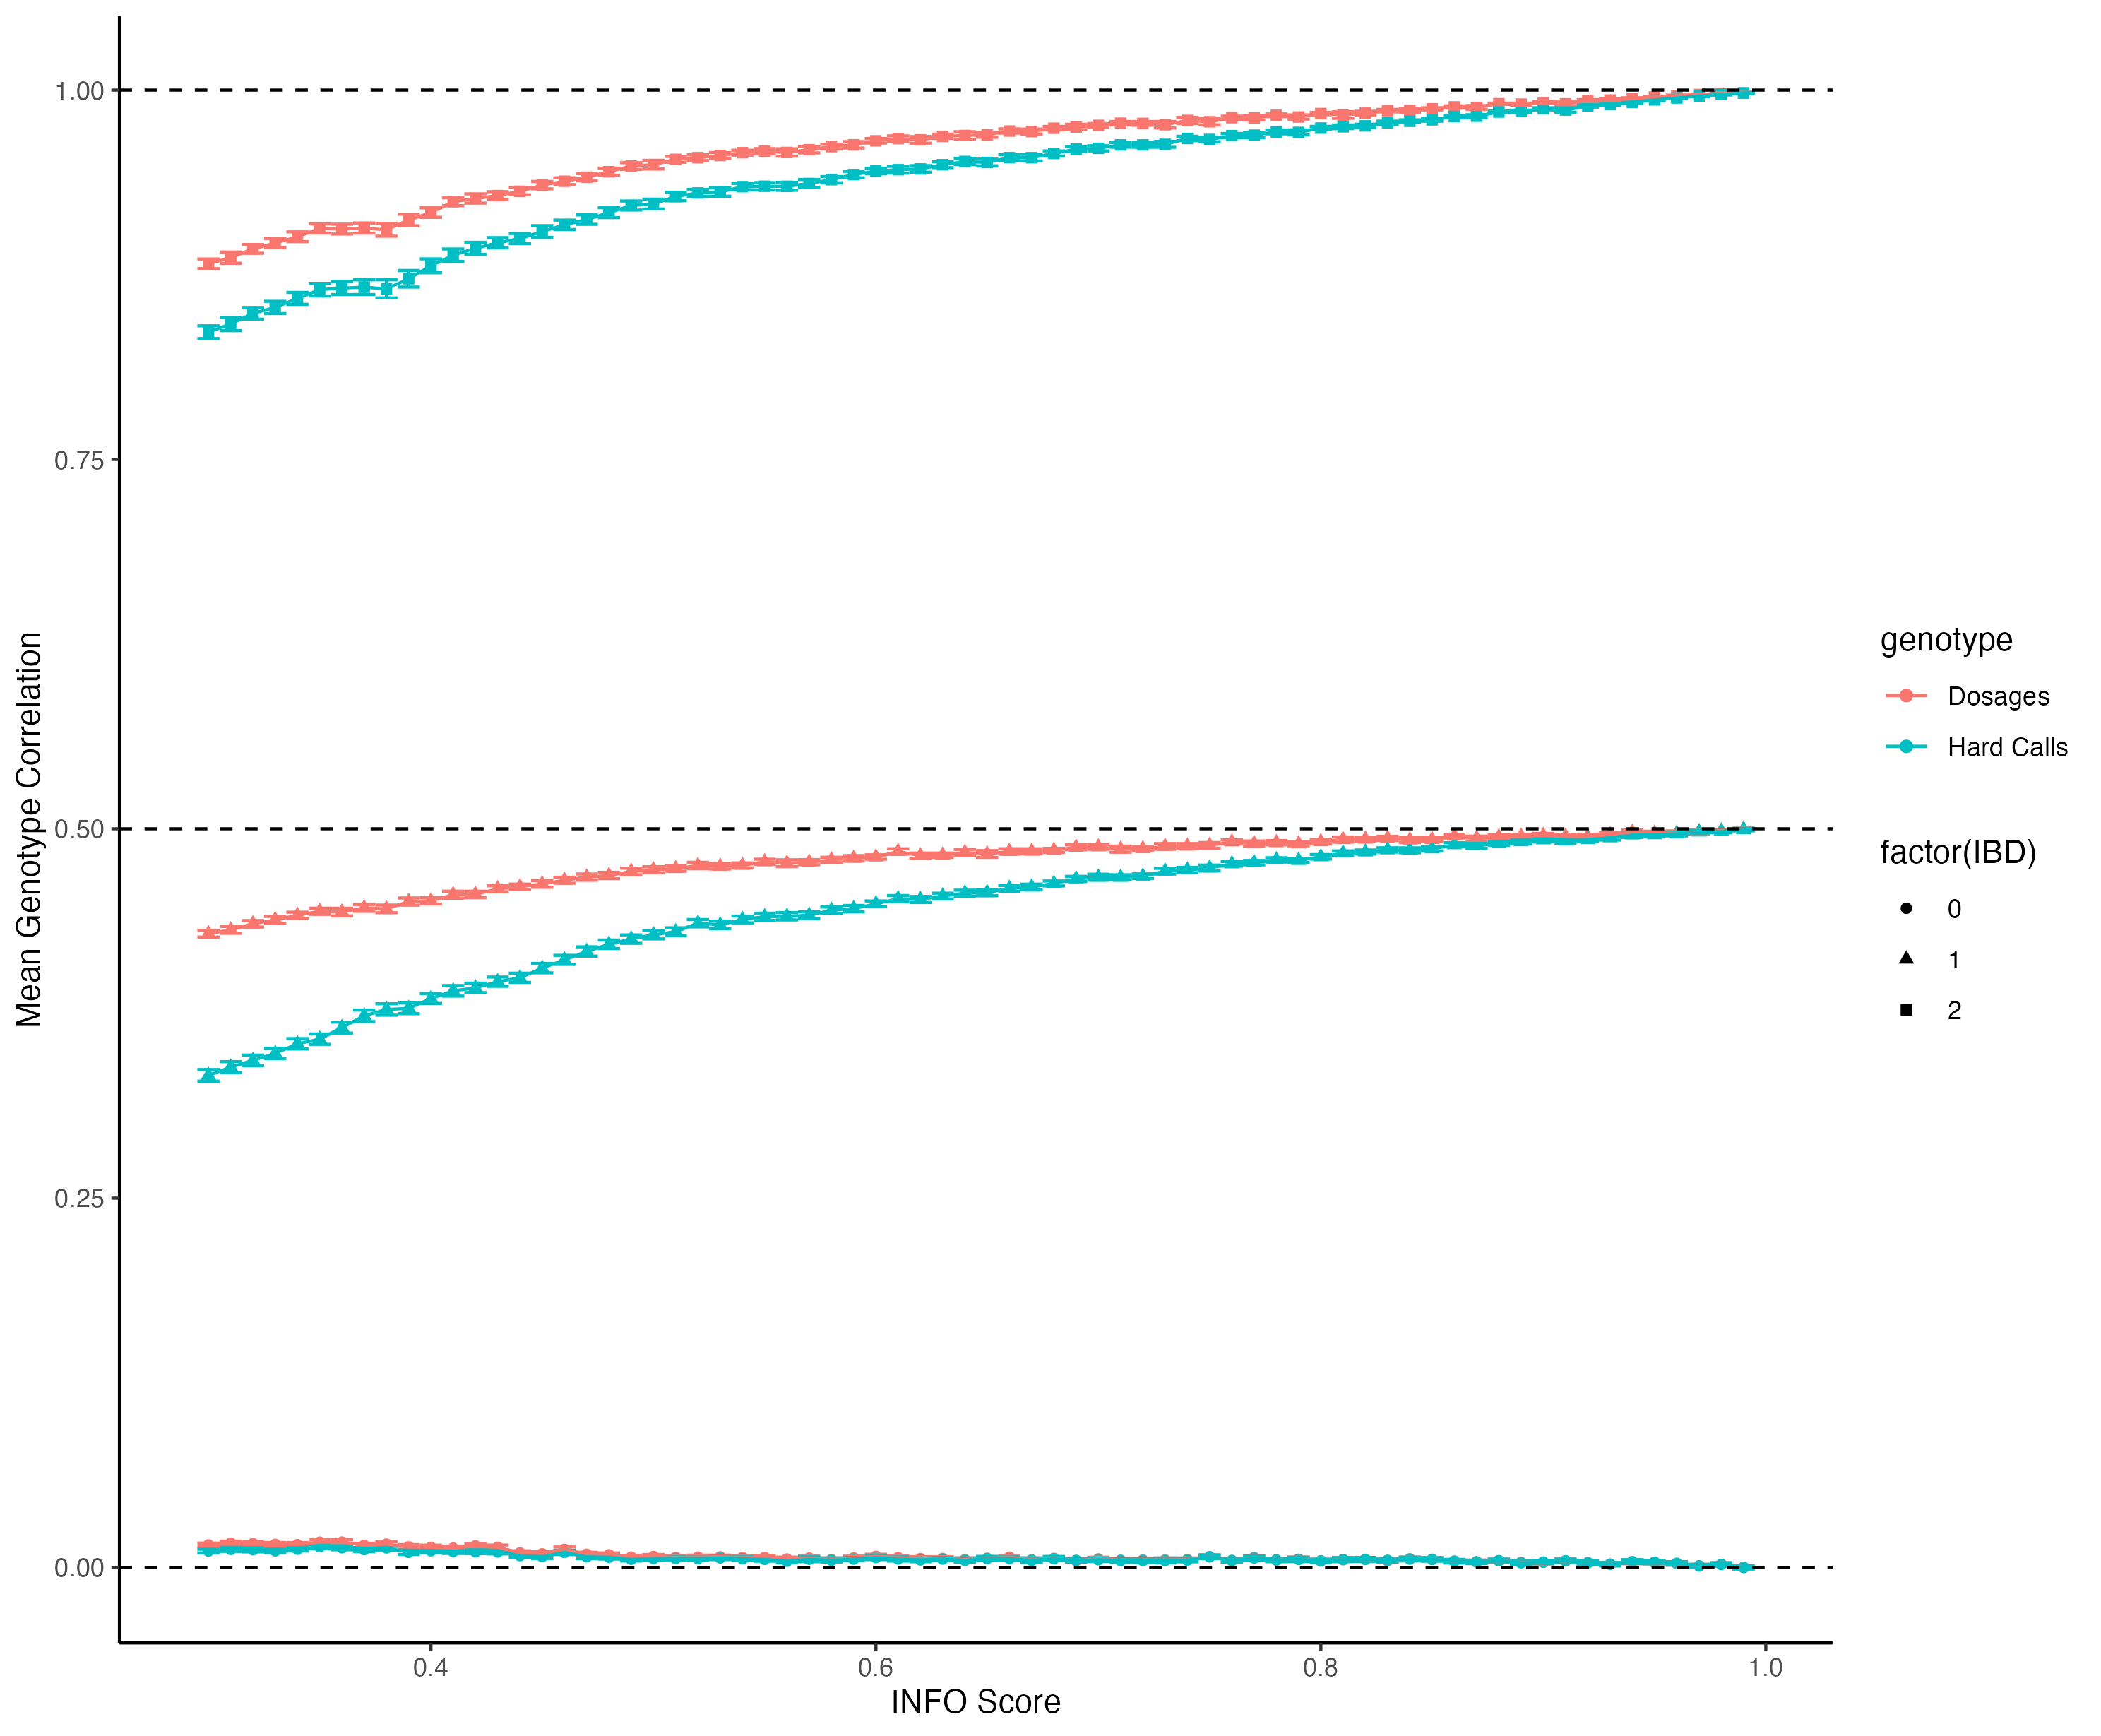
\includegraphics[width= .75\textwidth]{fig/mean_gt_by_ibd.png}
      \end{figure}
      % Briefly discuss the findings presented in this figure and their relevance.
      % add text to the figure adding the IBD state to the figure.
      % Under IBD 2 they should be perfectly correlated but as we see they are not.
      % under IBD 1 they should be correlated by 0.5 but as we see they are not.
      % and under IBD equal to zero they should not be correlated but as we see for low info scores they are weakly correlated.
\end{frame}


\begin{frame}{Next Steps}
      \begin{itemize}
            \item Using recently released WGS data from UKB. We are interesed to see what is the 
            the downstream effect of using low-quality imputed genotypes in Family-Based analysis.
            \vspace{10pt}
            \item We can do that by comparing the results of Family-Based analysis using imputed genotypes and the WGS data.
      \end{itemize}
\end{frame}

\begin{frame}{Conclusion}
    \begin{itemize}
      \item Genotyps imputed from a reference panel do not preserve Mandellian laws except for the very highest quality imputed variants.
      \vspace{10pt}
      \item This is worse for best guess (Hard Calls) genotypes than for dosages.
      \vspace{10pt}
      \item We are interested in developing reference-based imputation methods that take into account the relationships between the individuals.
    \end{itemize}
\end{frame}


\begin{frame}[plain]
      \centering
      \huge{Thank You!}
\end{frame}


\end{document}
